\documentclass[aspectratio=169, UTF8]{ctexbeamer}
\usetheme{Warsaw}
% \usetheme{split}
\usepackage{enumerate}
\usepackage{multirow}
\usepackage{multicol}
\usepackage[backend=biber,style=gb7714-2015, url=false, doi=true]{biblatex}
\usepackage{animate}
\usepackage{indentfirst}
\usepackage{booktabs}
\usepackage{subfigure}
\usepackage{listings}
\usepackage[dvipsnames]{xcolor}

\graphicspath{figures/}

% headline & footline
\setbeamertemplate{headline}{}

% 注释显示序号
\setbeamertemplate{caption}[numbered]

% 删除导航栏
\setbeamertemplate{navigation symbols}{}

% 页面显示编号


% 字族设置
\setCJKfamilyfont { ustc-song } {Source Han Serif CN}
\setCJKfamilyfont { ustc-hei  } {Source Han Sans SC}
\setCJKfamilyfont { ustc-kai  } {KaiTi_GB2312}
\setCJKfamilyfont { ustc-fangsong  } {FangSong_GB2312}
\setCJKfamilyfont { ustc-gengshahei  } {Sarasa Mono SC Nerd}
\NewDocumentCommand \ustcsong   { } { \CJKfamily { ustc-song  } }
\NewDocumentCommand \ustchei    { } { \CJKfamily { ustc-hei   } }
\NewDocumentCommand \ustckai   { } { \CJKfamily { ustc-kai   } }
\NewDocumentCommand \ustcfangsong   { } { \CJKfamily { ustc-fangsong   } }
\NewDocumentCommand \ustcgengshahei   { } { \CJKfamily { ustc-gengshahei   } }

%% 字体设置
\setCJKmainfont{Source Han Serif CN}
\setCJKsansfont{Source Han Sans SC}
% \setbeamerfont{author}{size=\}
\setbeamerfont{date}{size=\tiny}
\setbeamerfont{title}{series=\ustcsong\bfseries}
\setbeamerfont{subtitle}{series=\mdseries,size=\footnotesize}
\setbeamerfont{frametitle}{series=\sffamily\ustchei}
\setbeamerfont{framesubtitle}{series=\sffamily\ustchei}
\setbeamerfont{footline}{size=\scriptsize}
\setbeamerfont{block title}{series=\centering}
\setbeamerfont{block body}{family=\rmfamily}
\setbeamerfont{footnote}{size=\tiny,series=\ttfamily\slshape}


% 参考文献设置
\addbibresource{ref.bib}

\usepackage{caption}
% \captionsetup{font={tiny}}

\setlength{\parindent}{2em}

\setbeamertemplate{itemize item}[triangle]
\setbeamertemplate{itemize subitem}[circle]
\setbeamertemplate{itemize subsubitem}[square]

\setbeamertemplate{section in toc}[sections numbered]
\setbeamertemplate{subsection in toc}[subsections numbered]

\renewcommand*{\bibfont}{\footnotesize}

%% 代码设置
\lstset{
    language=Python, % 设置语言
 basicstyle=\ttfamily, % 设置字体族
 breaklines=true, % 自动换行
 keywordstyle=\bfseries\color{NavyBlue}, % 设置关键字为粗体,颜色为 NavyBlue
 morekeywords={}, % 设置更多的关键字,用逗号分隔
 emph={self}, % 指定强调词,如果有多个,用逗号隔开
    emphstyle=\bfseries\color{Rhodamine}, % 强调词样式设置
    commentstyle=\itshape\color{black!50!white}, % 设置注释样式,斜体,浅灰色
    stringstyle=\bfseries\color{PineGreen!90!black}, % 设置字符串样式
    columns=flexible,
    numbers=left, % 行号位置
    numbersep=2em, % 行号具体位置
    numberstyle=\footnotesize, % 缩小行号
    frame=single, % 边框
    framesep=1em % 设置代码与边框的距离
}
\author{汇报人 XXX\inst{1,2}
\newline  导师 XXX\inst{2}
}
\institute{
\inst{1}中国科学技术大学\quad XXXX系 
\newline \inst{2}中国科学院高能物理研究所
}
\date{XXXX年X月XX日}
\title{汇报标题}

\begin{document}

\begin{frame}
    \maketitle
\end{frame}

\begin{frame}{目录}
    \centering
    \tableofcontents[hideallsubsections]
\end{frame}

\section{第一章 XXXX}
\subsection{第一节 XXXX}

\begin{frame}{页标题}
    \begin{columns}
        \column{.45\paperwidth}
        \begin{block}{普通块}
            standard blocks
        \end{block}
        \begin{alertblock}{警示块}
            alert block
        \end{alertblock}
        \begin{exampleblock}{示例块}
            exampleb lock
        \end{exampleblock}
        \column{.45\paperwidth}
        \begin{theorem}
            Theorem
        \end{theorem}
        \begin{definition}
            Definition
        \end{definition}
        \begin{proof}
            Proof
        \end{proof}
    \end{columns}
    
\end{frame}

\begin{frame}{页标题}
    \begin{figure}
        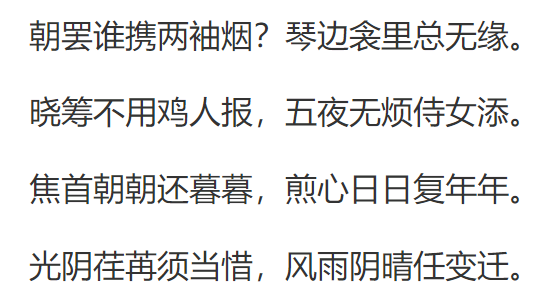
\includegraphics[height=0.6\textheight]{fig.png}
        \caption{灯谜}
    \end{figure}
\end{frame}

\section{第二章 XXXX}
\subsection{插入代码块}
\begin{frame}[fragile]{插入代码}{Insert Code Blocks}
    使用Listing宏包\begin{verbatim}
        \usepackage{listings}
    \end{verbatim}
    \begin{lstlisting}
        >>> import torch
        >>> print(torch.cuda.is_available())
        True
        >>> print(f'device name [0]:', torch.cuda.get_device_name(0))
        device name [0]: AMD Radeon RX 7900 XTX
    \end{lstlisting}
\end{frame}

\section[Reference Citations]{文献引用}
\subsection{文献引用}
\begin{frame}{文献引用脚注}{Reference Foot Citations}
    Xianguang et al.\footfullcite{WU2018281} conducted 2D wave tank tests in regular waves to evaluate the primary conversion efficiency of six kinds of BBDB models with different hull form. They showed that primary conversion efficiency of six kinds of models was 22\%~73\%. Lewis et al. \footfullcite{SHENG2019709} carried out 3D wave tank tests for a BBDB model with linear damper PTO simulator in regular waves and measured motions of BBDB and air pressure in air chamber etc. Forestier et al. \footfullcite{inproceedings} reported the results of wave tank tests and field tests for the power output of BBDB named “OEBuoy” by OceanEnergy Limited.
\end{frame}

\begin{frame}{文献引用}{Reference Citations}
    \printbibliography[heading=bibintoc]
    \insertframetitle
\end{frame}

\end{document}